% PolyU Beamer template demo — showcase of slide types (filler copy + sample assets)
% Build: pdflatex demo.tex  (run twice for TikZ overlays / TOC)
\documentclass[t]{beamer}
\usepackage[polyu,en]{collegeBeamer}
\usepackage{polyu_layout}
\usepackage{colortbl}

\title{Presentation Title:\\Second Line Goes Here}
\subtitle{\phantom{.}}
\author{Firstname Lastname\\Your Unit / Lab\\The Hong Kong Polytechnic University\\[8pt]Prof.\ Example Supervisor}
\date{\today}

\begin{document}

\maketitle

%=================================================================
\section{Context}

\begin{frame}{Two-column media}
  \textcolor{black}{\normalsize Lorem ipsum dolor sit amet, consectetur adipiscing elit.
  Highlight \ctextbf{key terms} in brand color.}

  \vspace{0.75em}
  \begin{columns}[c]
    \begin{column}{0.42\textwidth}
      \centering
      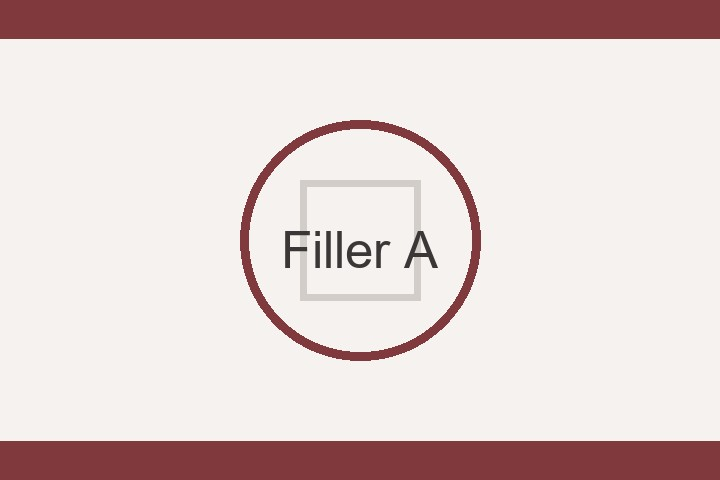
\includegraphics[width=0.92\linewidth,height=3.6cm,keepaspectratio]{gallery/dual_left.jpg}\\[0.3em]
      {\scriptsize\textcolor{black}{\textbf{Left caption}\\Short supporting line\\(optional detail)}}
    \end{column}
    \begin{column}{0.50\textwidth}
      \centering
      
\includegraphics[width=\linewidth,height=3.6cm,keepaspectratio]{gallery/dual_right.png}\\[0.3em]
      {\scriptsize\textcolor{black}{\textbf{Right caption}\\Short supporting line\\(optional detail)}}
    \end{column}
  \end{columns}
\end{frame}

\begin{frame}{Numbered points + figure}
  \begin{enumerate}
    \item Lorem ipsum dolor sit amet --- \textit{emphasized clause}.
    \item Sed do eiusmod tempor incididunt ut labore et dolore.
    \item Ut enim ad minim veniam, quis nostrud exercitation.
  \end{enumerate}

  \vspace{0.5em}
  \centering
  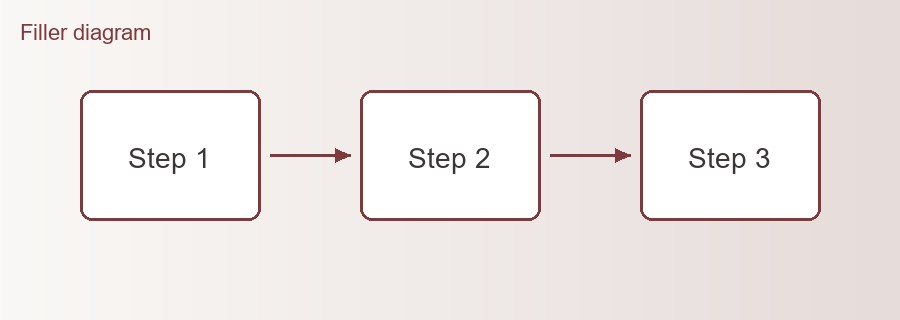
\includegraphics[width=0.60\textwidth,height=2.35cm,keepaspectratio]{gallery/flow.jpg}
\end{frame}

\begin{frame}{Bullet list}
  \begin{itemize}
    \item First supporting point with enough length to wrap if needed
    \item Second point referencing a \ctextbf{branded} phrase
    \item Third point --- keep one idea per bullet
    \item Optional fourth point for density check
  \end{itemize}
\end{frame}

\begin{frame}[c]
  \centerstate{
    \Large
    One-line thesis or provocation,\\[0.45em]
    centered for emphasis,\\[0.45em]
    with a \ctextbf{brand} accent.
  }
\end{frame}

\begin{frame}{List + image grid}
  \begin{columns}[T]
    \begin{column}{0.46\textwidth}
      \textbf{Group A}
      \begin{itemize}
        \item Item Alpha
        \item Item Beta
        \item Item Gamma
      \end{itemize}
      \vspace{0.35em}
      \textbf{Group B}
      \begin{itemize}
        \item Item Delta
        \item Item Epsilon
        \item Item Zeta
      \end{itemize}
    \end{column}
    \begin{column}{0.52\textwidth}
      \centering
      \begin{tikzpicture}[x=1cm,y=1cm]
        \node[inner sep=0] at (0.00, 1.90)
          {
\includegraphics[width=3.15cm]{gallery/venues/nhb.png}};
        \node[inner sep=0] at (3.45, 1.90)
          {
\includegraphics[width=3.15cm]{gallery/venues/ncomms.png}};
        \node[inner sep=0] at (0.00, 0.35)
          {
\includegraphics[width=3.15cm]{gallery/venues/npjdm.png}};
        \node[inner sep=0] at (3.45, 0.35)
          {
\includegraphics[width=3.15cm]{gallery/venues/sleep.png}};
        \node[inner sep=0] at (0.00,-1.20)
          {
\includegraphics[width=3.15cm]{gallery/venues/jsr.png}};
        \node[inner sep=0] at (3.45,-1.20)
          {
\includegraphics[width=3.15cm]{gallery/venues/srep.png}};
      \end{tikzpicture}
    \end{column}
  \end{columns}
\end{frame}

\begin{frame}{Dual cards}
  \centering
  {\normalsize Short headline above the cards}

  \vspace{0.85em}
  \begin{columns}[T]
    \begin{column}{0.48\textwidth}
      \centering
      \drawcard{Card A --- Label}{%
        Short body line one\\[0.15em]
        Short body line two%
      }{5.2cm}
    \end{column}
    \begin{column}{0.48\textwidth}
      \centering
      \drawcard{Card B --- Label}{%
        Short body line one\\[0.15em]
        Short body line two%
      }{5.2cm}
    \end{column}
  \end{columns}
\end{frame}

%=================================================================
\section{Layouts}

\begin{frame}[c]{Centered question}
  \centerstate{
    \Large
    How should we frame the\\[0.45em]
    \ctextbf{core question} on this slide?
  }
\end{frame}

\begin{frame}{Simple table}
  \plaintable{%
    \small
    \renewcommand{\arraystretch}{1.25}
    \begin{tabularx}{\linewidth}{@{}>{\raggedright\arraybackslash}X
      >{\raggedright\arraybackslash}X
      >{\raggedright\arraybackslash}X@{}}
      \toprule
      \textbf{Column A} & \textbf{Column B} & \textbf{Column C} \\
      \midrule
      Row one & Value & Value \\
      Row two & Value & Value \\
      Row three & Value & Value \\
      \bottomrule
    \end{tabularx}%
  }
\end{frame}

\begin{frame}[shrink=10]{Text + session sketch + image}
  \studypair{%
      \small
      \textbf{Lead-in:} short framing sentence for the block on the left.

      \vspace{0.28em}
      \sessionsketch
        {Short design line · optional detail}
        {Option A vs Option B, brief note}
        {Step one $\rightarrow$ step two $\rightarrow$ step three}
        {Item one, item two, optional item}

      \vspace{0.28em}
      \plaintable{%
        \renewcommand{\arraystretch}{1.02}
        \begin{tabularx}{\linewidth}{@{}lX@{}}
          \toprule
          Label & Detail \\
          \midrule
          Row A & Short placeholder \\
          Row B & Short placeholder \\
          Row C & Short placeholder \\
          \bottomrule
        \end{tabularx}%
      }
  }{gallery/paired_fill.jpg}
\end{frame}

\begin{frame}{Roadmap strips}
  \roadmaprows{
    0/{\textbf{Align} \quad Decide scope and first deliverable.},
    1/{\textbf{Gather} \quad Collect low-cost data and references.},
    2/{\textbf{Pilot} \quad Run a small controlled check ($N\sim$12--20).},
    3/{\textbf{Scale} \quad Repeat the same protocol with a larger audience.},
    4/{\textbf{Write} \quad Draft findings (one paper or separate notes).}
  }
\end{frame}

\begin{frame}[shrink=5]{Text + small image}
  \studypairsm{0.64\textwidth}{0.26\textwidth}{%
      \small
      \textbf{Lead-in:} short framing sentence.

      \vspace{0.35em}
      \begin{itemize}
        \item Bullet one
        \item Bullet two
        \item Bullet three
      \end{itemize}

      \vspace{0.3em}
      Optional closing line.
  }{gallery/paired_sm.png}
\end{frame}

\begin{frame}{Table + image}
  \studypairxy{0.58\textwidth}{0.38\textwidth}{%
      \plaintable{%
        \scriptsize
        \renewcommand{\arraystretch}{1.15}
        \begin{tabularx}{\linewidth}{@{}>{\bfseries}l X@{}}
          \toprule
          Label A & Short placeholder text \\
          Label B & Short placeholder text \\
          Label C & Short placeholder text \\
          Label D & Short placeholder text \\
          Label E & Short placeholder text \\
          Label F & Short placeholder text \\
          \bottomrule
        \end{tabularx}%
      }%
  }{gallery/phase_fill.jpg}
\end{frame}

\QApage

\end{document}
